\subsection{情報の流れ}
本システムは、管理者サーバー・データベースを中心に、利用者(依頼者)・配達員・サービス加盟店(店舗)によって構成されている。図\ref{system}~図\ref{money}に情報および金銭の流れを示す。図6,7は情報の流れ、図8は金銭の流れを表している。
本システムでは、利用者がアプリ上で商品を注文すると、注文情報がサーバーを介して店舗および配達員に送信される。配達員は受注内容に基づき店舗から商品を受け取り、指定の配達先まで配送を行う。配達完了後、店舗および配達員はそれぞれシステムに配送完了報告を送信し、管理サーバーで取引が確定する。

\begin{figure}[H]
  \centering
  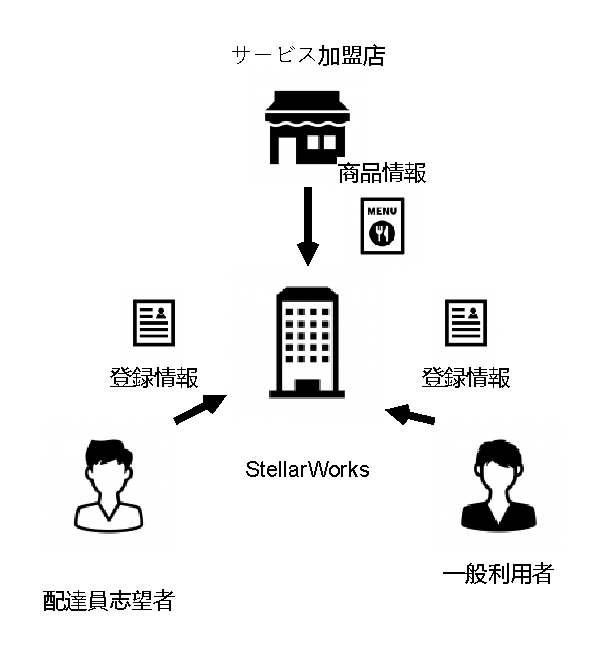
\includegraphics[width=0.5\textwidth]{情報の流れ.drawio.pdf}
  \caption{情報の流れ: 情報登録}
  \label{system}
\end{figure}

\begin{figure}[H]
  \centering
  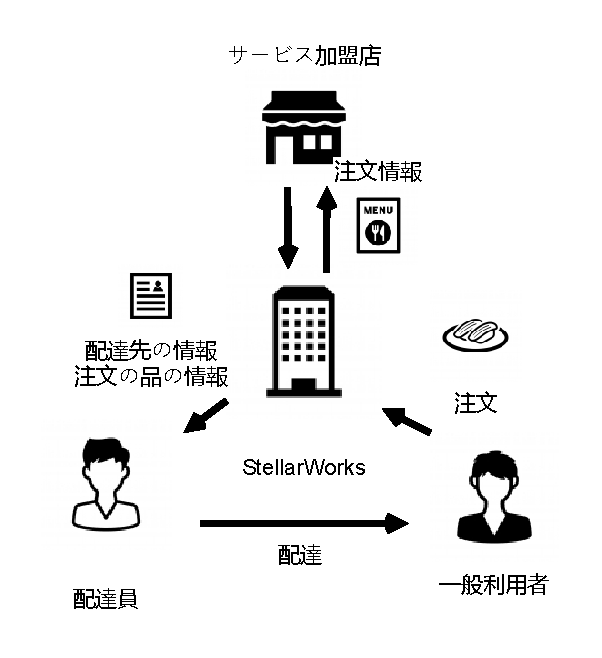
\includegraphics[width=0.5\textwidth]{流れ.drawio.pdf}
  \caption{情報の流れ: 注文から配達まで}
  \label{oder}
\end{figure}


\subsection{金銭の流れ}
本システムの金銭の流れは以下の通りである。
支払い方式は銀行振り込みによる月末一括精算方式を採用している。利用者(依頼者)は、当月内の利用分について月末にまとめて銀行振り込みで支払いを行う。
また、クレジットカードを用いたオンライン決済システムも導入しており、利用者はアプリ上でクレジットカード情報またはkamicaなどの情報を登録し、月末に自動的に決済が行われる仕組みとなっている。
運営側は決済代行システムを通じて支払いを一元管理し、店舗・配達員への報酬支払いを翌月初めに一括処理する。
これにより、個々の取引ごとに発生していた送金処理を効率化し、運用コストを削減している。
また、配達員は商品を受け取る際に自らの手持ち資金を使用しないため、商品が売り切れなどの不測の事態が発生しても払い戻しが三者間で発生しない仕組みとなっている。
利用者は返金や精算の手間をかけることなく、快適にシステムを利用できる。
このように、本システムは銀行振り込み機能を用いることで、取引の透明性と効率性を両立した金銭管理体制を実現している。
\begin{figure}[H]
  \centering
  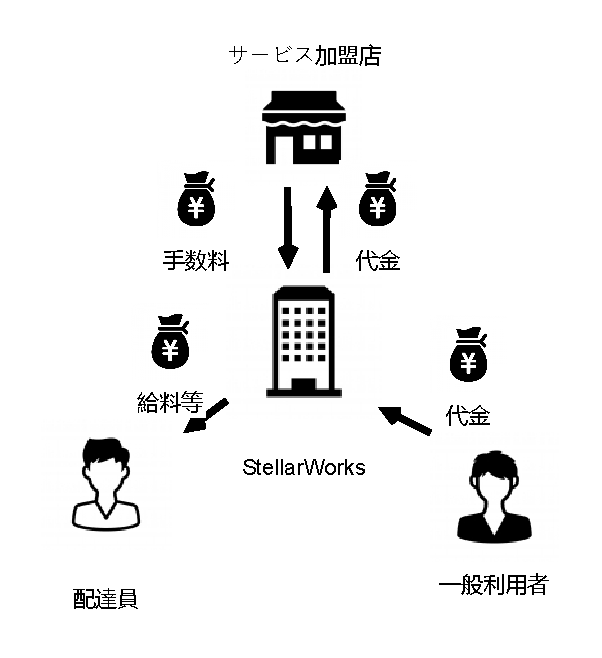
\includegraphics[width=0.5\textwidth]{お金の流れ1.pdf}
  \caption{金銭の流れ}
  \label{money}
\end{figure}
